\documentclass[APA,LATO1COL,doublespace]{WileyNJD-v2}
\usepackage{moreverb}

% Giuliano
\usepackage{graphicx}
\graphicspath{ {Figures/} }
\usepackage{enumitem} % to have (i) bulletts
\usepackage[margins]{trackchanges}
%
% ==== REVIEW ONLY ====
% http://texdoc.net/texmf-dist/doc/latex/endfloat/endfloat.pdf
% tables and figures at the end of document
\usepackage[notablist,figlist,tablesfirst]{endfloat}
% =====================
%
% == COMMENT AFTER EDITOR APPROVAL ABOUT LENGTH OF PAPER ==
%\usepackage{draftwatermark}
%\SetWatermarkText{Ed. approval}
%\SetWatermarkScale{1.0} % size of the watermark
% =========================================================
%
% ==== ADD ORCID REFERENCE ====
% git repo :: https://github.com/diogo-fernan/academicons
%
%    **ATTEMPT #1**
% See link https://tex.stackexchange.com/questions/275578/is-there-a-standard-way-to-include-orcid-in-tex-pdf
%\usepackage{./academicons}
%\newcommand{\myOrcid}[1]{\href{https://orcid.org/#1}{\textcolor[HTML]{A6CE39}{\aiOrcid}}}
%\definecolor{orcidlogocol}{HTML}{A6CE39}
%
%    **ATTEMPT #2**
% https://tex.stackexchange.com/questions/445563/ieeetran-how-to-include-orcid-in-tex-pdf-with-pdflatex
\usepackage{scalerel}
\usepackage{tikz}
\usetikzlibrary{svg.path}
\definecolor{orcidlogocol}{HTML}{A6CE39}
\tikzset{
  orcidlogo/.pic={
    \fill[orcidlogocol] svg{M256,128c0,70.7-57.3,128-128,128C57.3,256,0,198.7,0,128C0,57.3,57.3,0,128,0C198.7,0,256,57.3,256,128z};
    \fill[white] svg{M86.3,186.2H70.9V79.1h15.4v48.4V186.2z}
                 svg{M108.9,79.1h41.6c39.6,0,57,28.3,57,53.6c0,27.5-21.5,53.6-56.8,53.6h-41.8V79.1z M124.3,172.4h24.5c34.9,0,42.9-26.5,42.9-39.7c0-21.5-13.7-39.7-43.7-39.7h-23.7V172.4z}
                 svg{M88.7,56.8c0,5.5-4.5,10.1-10.1,10.1c-5.6,0-10.1-4.6-10.1-10.1c0-5.6,4.5-10.1,10.1-10.1C84.2,46.7,88.7,51.3,88.7,56.8z};
  }
}
\newcommand\orcidicon[1]{\href{https://orcid.org/#1}{\mbox{\scalerel*{

\begin{tikzpicture}[yscale=-1,transform shape]
\pic{orcidlogo};
\end{tikzpicture}
}{|}}}}
\usepackage{hyperref} %<--- Load after everything else
% =============================
%
%\usepackage{array}
%\usepackage{cleveref}
%\usepackage{siunitx}

\newcommand\BibTeX{{\rmfamily B\kern-.05em \textsc{i\kern-.025em b}\kern-.08em
T\kern-.1667em\lower.7ex\hbox{E}\kern-.125emX}}

\articletype{Research Article}%

\received{<day> <Month>, <year>}
\revised{<day> <Month>, <year>}
\accepted{<day> <Month>, <year>}

%\raggedbottom

\begin{document}

\title{Soil Monitor: an internet platform to challenge soil sealing in Italy}

\author[1,2]{Giuliano Langella*}
\author[2,3]{Angelo Basile}
\author[4]{Simone Giannecchini}
\author[5,6]{Francesco Domenico Moccia}
\author[1]{Florindo Antonio Mileti}
\author[7]{Michele Munaf\'o}
\author[8]{Francesco Pinto}
\author[1,2]{Fabio Terribile}
\authormark{LANGELLA \textsc{et al}}

%\address[1]{\orgdiv{Org Division}, \orgname{Org name}, \orgaddress{\state{State name}, \country{Country name}}}
\address[1]{\orgdiv{Department of Agriculture}, \orgname{Universit\'a di Napoli Federico II}, \orgaddress{via Universit\'a 100, Portici 80055, \state{Napoli}, \country{Italy}}}

\address[2]{\orgdiv{Interdepartmental Centre on Earth Critical Zone (CRISP)}, \orgname{Universit\'a di Napoli Federico II}, \orgaddress{via Universit\'a 100, Portici 80055, \state{Napoli}, \country{Italy}}}

\address[3]{\orgdiv{ISAFom Institute}, \orgname{National Research Council}, \orgaddress{via Patacca 85, Ercolano 80056, \state{Napoli}, \country{Italy}}}

\address[4]{\orgname{GeoSolutions S.A.S.}, \orgaddress{via di Montramito 3/A, Massarosa 55054, \state{Lucca}, \country{Italy}}}

\address[5]{\orgdiv{Department of Architecture}, \orgname{Universit\'a di Napoli Federico II}, \orgaddress{via Toledo 402, Napoli 80134, \state{Napoli}, \country{Italy}}}

\address[6]{\orgname{Istituto Nazionale di Urbanistica (INU)}, \orgaddress{Via Castro dei Volsci 14, Roma 00179 \state{Roma}, \country{Italy}}}

\address[7]{\orgname{Istituto Superiore per la Protezione e la Ricerca Ambientale (ISPRA)}, \orgaddress{Via Brancati 48, Roma 00144 \state{Roma}, \country{Italy}}}

\address[8]{\orgname{EMM S.R.L.}, \orgaddress{via Vicinale Santa Maria del Pianto, Napoli 80143 \state{Napoli}, \country{Italy}}}


\corres{*Giuliano Langella, Department of Agriculture, Universit\'a di Napoli Federico II. \email{glangella@unina.it}}

\presentaddress{via Universit\'a 100, 80055 Portici, Italy}


\abstract[Abstract]{ 
This work aims to show that a new type of web-based geospatial Decision Support System --- Soil Monitor application (SMapp, www.soilmonitor.it), developed on top of open-source Geospatial Cyber-Infrastructures (GCI) --- can provide a multidisciplinary operational tool useful for a multi-stakeholder community to challenge soil sealing.
Different technological and technical features of SMapp are presented and discussed with particular reference to the combination of WebGIS with on-the-fly geospatial processing based on GPU computing, specifically designed, developed, and embedded in the presented GCI allowing real-time requests.
Soil Monitor is shown as operational in three different case studies, which are also different scales where policy making and decisions about measures to tackle land take are entangled, at least in Italy.
Accordingly, examples of soil sealing indicators are presented, such as an interactive Land Use and Land Cover (LULC) matrix and the map of rural fragmentation.
As a result, SMapp models are deemed useful to (i) support decision making, (ii) raise awareness in people, professionals, and experts of other fields, and (iii) contrastingly put current law in force and actual land take situation owing to multitemporal datasets as an ex post control tool.
The pros and cons are discussed with special emphasis on the limits (new codes from scratch) and benefits (low-cost, low-energy fast computing) from the use of codes and primitives for land degradation written in CUDA (Compute Unified Device Architecture): a library to maintain and develop further in order to success in facing land take, according to the zero land take deadlines.
}

\keywords{soil sealing, geospatial decision support system, CUDA, GPU computing, urban planning}
%Class file; \LaTeXe; \emph{Wiley NJD}}

\jnlcitation{
\cname{%
    \author{Langella G.}, 
    \author{A. Basile}, 
    \author{S. Giannecchini}, 
    \author{F.D. Moccia}, 
    \author{F.A. Mileti},
    \author{M. Munaf\'o},
    \author{F. Pinto} and
    \author{F. Terribile}
}
(\cyear{<year>}), 
\ctitle{Soil Monitor: an internet platform to challenge soil sealing in Italy},
\cjournal{Land Degradation \& Development}, \cvol{<year>;<number>:<page>--<page>}.}

\maketitle

%\footnotetext{\textbf{Abbreviations:} ANA, anti-nuclear antibodies; APC, antigen-presenting cells; IRF, interferon regulatory factor}

\section{Introduction}\label{sec1}
Soil sealing is one of the most serious land degradation process, which refers to covering the ground by an impermeable material.
It is regarded as the greatest threat to soil functions since it strongly disturbs or removes essential ecosystem services such as food production, water absorption, rainwater infiltration, and groundwater recharge, filtering and buffering capacity of the soil, biodiversity, etc. \citep{FAO15}.
Accordingly, several services of such kind are irreplaceable, such as those provided and supported by healthy soils and diverse vegetation \citep{Dunbar13}.
According to the European Environmental Agency \citep{EEA2011}, land take (land converted into artificial surfaces) by cities has increased by about 80\% in the past 60 years (whereas population has grown by only 33\%); thus, soil sealing and land take are the most important issues reducing irreplaceable ecosystem services.

Several European policy documents have been produced to tackle the loss of ecosystem services as well as the restoration and maintenance thereof, such as the Habitats (92/43/EEC) and Birds (2009/147/EC) Directives, the Common Agriculture Policy (CAP), and the EU Biodiversity Strategy to 2020 (specifically, Target 2).
In addition to the general regulatory frameworks, important policy measures specifically dealing with ecosystem services provided by soil functions include the Thematic Strategy for Soil Protection \citep{EC2006} and implementation of the Strategy \citep{EC2012}; the Roadmap to a Resource Efficient Europe \citep{EC2011a} targeted to limit the yearly land take at the EU level by 2020 and aiming to achieve the zero net land take by 2050 in line with the RIO conference in 2012; the delivery of guidelines of good practices to mitigate soil sealing \citep{SWD12}; the delivery of the United Nations agenda \citep{UN15} for sustainable development goals, specifically Goal 11 ''\textit{Make cities and human settlements inclusive, safe, resilient, and sustainable}'' \citep{Keesstra16}.
Despite the large list of regulatory frameworks, there are no signs of change at present, and soil sealing continues to increase annually \citep{FAO15} at global (e.g. Secretariat of the Convention on Biological Diversity, 2012; UN, 2014), European (e.g. \citealp{SWD12}), and national scales \citep[e.g.][Copernicus Land Monitoring Service\footnote{ http://land.copernicus.eu}]{ISPRA16,ISPRA18}.
Moreover, the causes for soil sealing are very diverse and possible actions strongly depend on where they should be taken.

In the last decade, research on soil sealing has attempted to contribute to the understanding of this challenging soil degradation process. Major effort has been undertaken for the development of suitable monitoring methodologies \citep{ISPRA18,Alvarado18} and the evaluation of the impacts over the loss of soil ecosystem services \citep{Calzolari16}. Differently, limited effort has gone into developing operational spatial decision support tools addressing soil sealing.
This situation is unfortunate considering that there is a growing body of applications illustrating the utility of the geospatial decision support system (SDSS) and visualization tools for spatial and urban planning  \citep[e.g.][]{Bishop98,Geertman12,Carsjens07,Malczewski04,Malczewski06,Meyer08}.
In most cases, these SDSS have been conceived and developed to address small geographical areas, such as the SDSS proposed by \citep{Piero17} for 13 municipalities in South Italy, or for solving few, if not one, specific problems \citep[e.g.][]{Fedra98,Meyer08,Torresan16}. %(e.g. Fedra \& Feoli, 1998; Meyer \& Grabaum, 2008; Torresan et al., 2016).

Moreover, few contributions have clearly identified that urban planning DSS must include predictive scenario analysis \citep{Choi16,Xiang03,Volk10} and the \textit{what-if} modelling. In fact, this is very much required in planning procedures in order to design and evaluate the potential impact of alternative urban/rural spatial plans \citep{Hawkins02,Harms95,Choi16,vonHaaren06}. 
Furthermore, scenario analysis is crucial in Strategic Environmental Assessment (e.g. SEA and EIA EU Directives). Currently, this fundamental planning procedure is dominated by qualitative assessment methods while there is a great demand for objective and quantitative methods \citep{Choi16} to provide more accurate and quantitative predictions of the impact of a plan or project \citep{Carver03,Vanderhaegen05}.

A decision support system addressing soil sealing should rely on well-established models, algorithms, and indicators. The use of indicators to monitor and assess soil sealing is already well known \citep{King16}, and there has been a proliferation of indicators, metrics, reports, community indicators, state of the art reports, and assessment reports, etc. \citep{Maclaren96,Tanguay10}.
In addition, specific spatial resolution requirements of indicators have been greatly emphasised \citep{Jaeger08}.
Furthermore, a large set of soil sealing indicators is typically tuned to the specific geographic, environmental, and socio-economic setting under investigation.
For instance, \citet{Munafo13}, analysed the Italian territory and identified soil sealing trends in relation to the distance from the coastline or the elevation belt, to the land cover classes or the distance from neighbour urban patches.
Accordingly, references to soil sealing indicators and best practices regarding producing them in different EU countries have been reported in \citep{EC2011b} in which, for instance, the monitoring of built areas, the total amount of green areas within city boundaries, and the unpaved land areas can be found.

Consequently, it is evident that 
(i) action is required since ``future generations will not see a healthy soil coming back within their lifetime once it has been destroyed\dots'' \citep{SWD12}; 
(ii) soil sealing mitigation must embody urban and landscape planning tools \citep{Artmann14}, enabling the link of opposite socio-economic driving forces, such as urban regeneration versus environmental protection; 
(iii) inter- and trans-disciplinary studies integrating soils in the environment are required to challenge soil sealing;
(iv) a cross-topic awareness should be raised regarding soil sealing in the policy, research, and public sectors; 
and (v) there is a strong gap in building/providing integrated operational tools to support decision making over soil sealing for large areas, and the situation is even more difficult, considering that these tools --- to be properly operated by planners --- should also enable scenario analysis (\textit{what-if} modelling).

The general aim of this paper is to demonstrate that a new type of geospatial DSS --- a web-based DSS, namely Soil Monitor application (SMapp) --- developed on top of Geospatial Cyber-Infrastructures (GCI), can provide a multidisciplinary operational tool useful for a multi-stakeholder community to challenge soil sealing at the entire Italian country scale. 
This system is designed to address the accountancy of soil sealing through different indicators providing operational support to urban planners, decision makers and multi stakeholders involved in landscape planning and interested in evaluating the impact of soil sealing. 
This specific contribution required a different approach, the result of which is the Soil Monitor web application. 
A set of indicators can be calculated in real-time using either Italian administrative levels (NUTS2, NUTS3, and LAU2) or user-drawn Regions of Interest (RoI). 
Moreover, Soil Monitor uses high resolution layers produced every year by ISPRA (Italian Institute for Environmental Protection and Research) since 2015 for drawing up the yearly soil sealing report in Italy. 
Thus, owing to the high-performance computing embedded in its cyber infrastructure, Soil Monitor enables real-time geospatial processing while preserving a high spatial detail of the analysis over large areas (till LAU2); this combination of features has an intrinsic vast potential for being used in operational spatial planning. 

\section{ \change[GL]{Soil Monitor application (SMapp)} { Materials and Methods } }
\subsection{Design}
The Soil Monitor spatial decision support system and visualization tools are required to embody some crucial design items. 
Although the first version of the implementation was carried out without great involvement of stakeholders, because of money, time, and manpower constraints, at least two middle phases of consultation managed to apply modifications to the SMapp design and functionality. 
These consultations were performed with INU (National Institute for Urban planning) and ISPRA, which are the most important spatial planners' association in Italy along with being the public authority competent in monitoring land degradation and soil sealing, respectively.

Accordingly, the early stage design considerations included (i) the use of national scale standardized soil imperviousness high resolution layers, which is crucial since it avoids subjective soil sealing classification and very coarse soil sealing quantification as those using only the Corine Land Cover dataset; (ii) the use of fully transparent processing engines in order to provide the user a complete understanding of the data output; (iii) the use of open-source approaches to better tune this system to FAIR (Findability, Accessibility, Interoperability, and Reusability) data ; (iv) addressing high demanding computing needs.

The last issue mentioned above is critical because the wrapping of some algorithms in our platform is rather challenging, such as the scenario analysis that, for instance, computes --- through the web and on-the-fly --- metrics related to the change of rural fragmentation after a new urban setting is applied.
Moreover, encapsulating soil sealing models and indicators using an HPC (High Performance Computing) approach to both allow fast calculations and speed up the decision-making process. Consequently, the choice was for (i) a parallel computing platform based on graphics cards (GPU computing) using the NVIDIA hardware and software framework called CUDA (Compute Unified Device Architecture); (ii) implementing stand-alone CUDA-C codes allowing geospatial GPU based processing; (iii) wrapping the PTX CUDA kernels, after compiling CUDA-C source code, through the JAI-JCuda-CUDA chain. This specific choice is critical considering the high potential evolution of GPU technologies with respect to standard CPU approaches, also including the continual increase in the availability of these resources over the cloud. 
Furthermore, it was fundamental to manage both a multi-domain RoI definition and multi-user soil sealing platform.

\subsection{System architecture}
Soil Monitor\footnote{\emph{www.soilmonitor.it}} is currently in use and active within the Italian administrative boundaries (Figure \ref{fig:SMapp}).
It is based on free open-source geospatial libraries and programs and enables users to interact directly with the geospatial data on the map via the web.
Additionally, it has been developed starting from modular open-source codes specifically designed to create, manage, and share different types of geospatial information in a rather safe, simple, and intuitive way.
In particular, SMapp is deployed on the dual infrastructure GeoServer and MapStore, the both of which are mainly developed and maintained worldwide by GeoSolutions.

\begin{figure}[t]
    % \includegraphics[width,,height=15pc,draft]
    \centerline{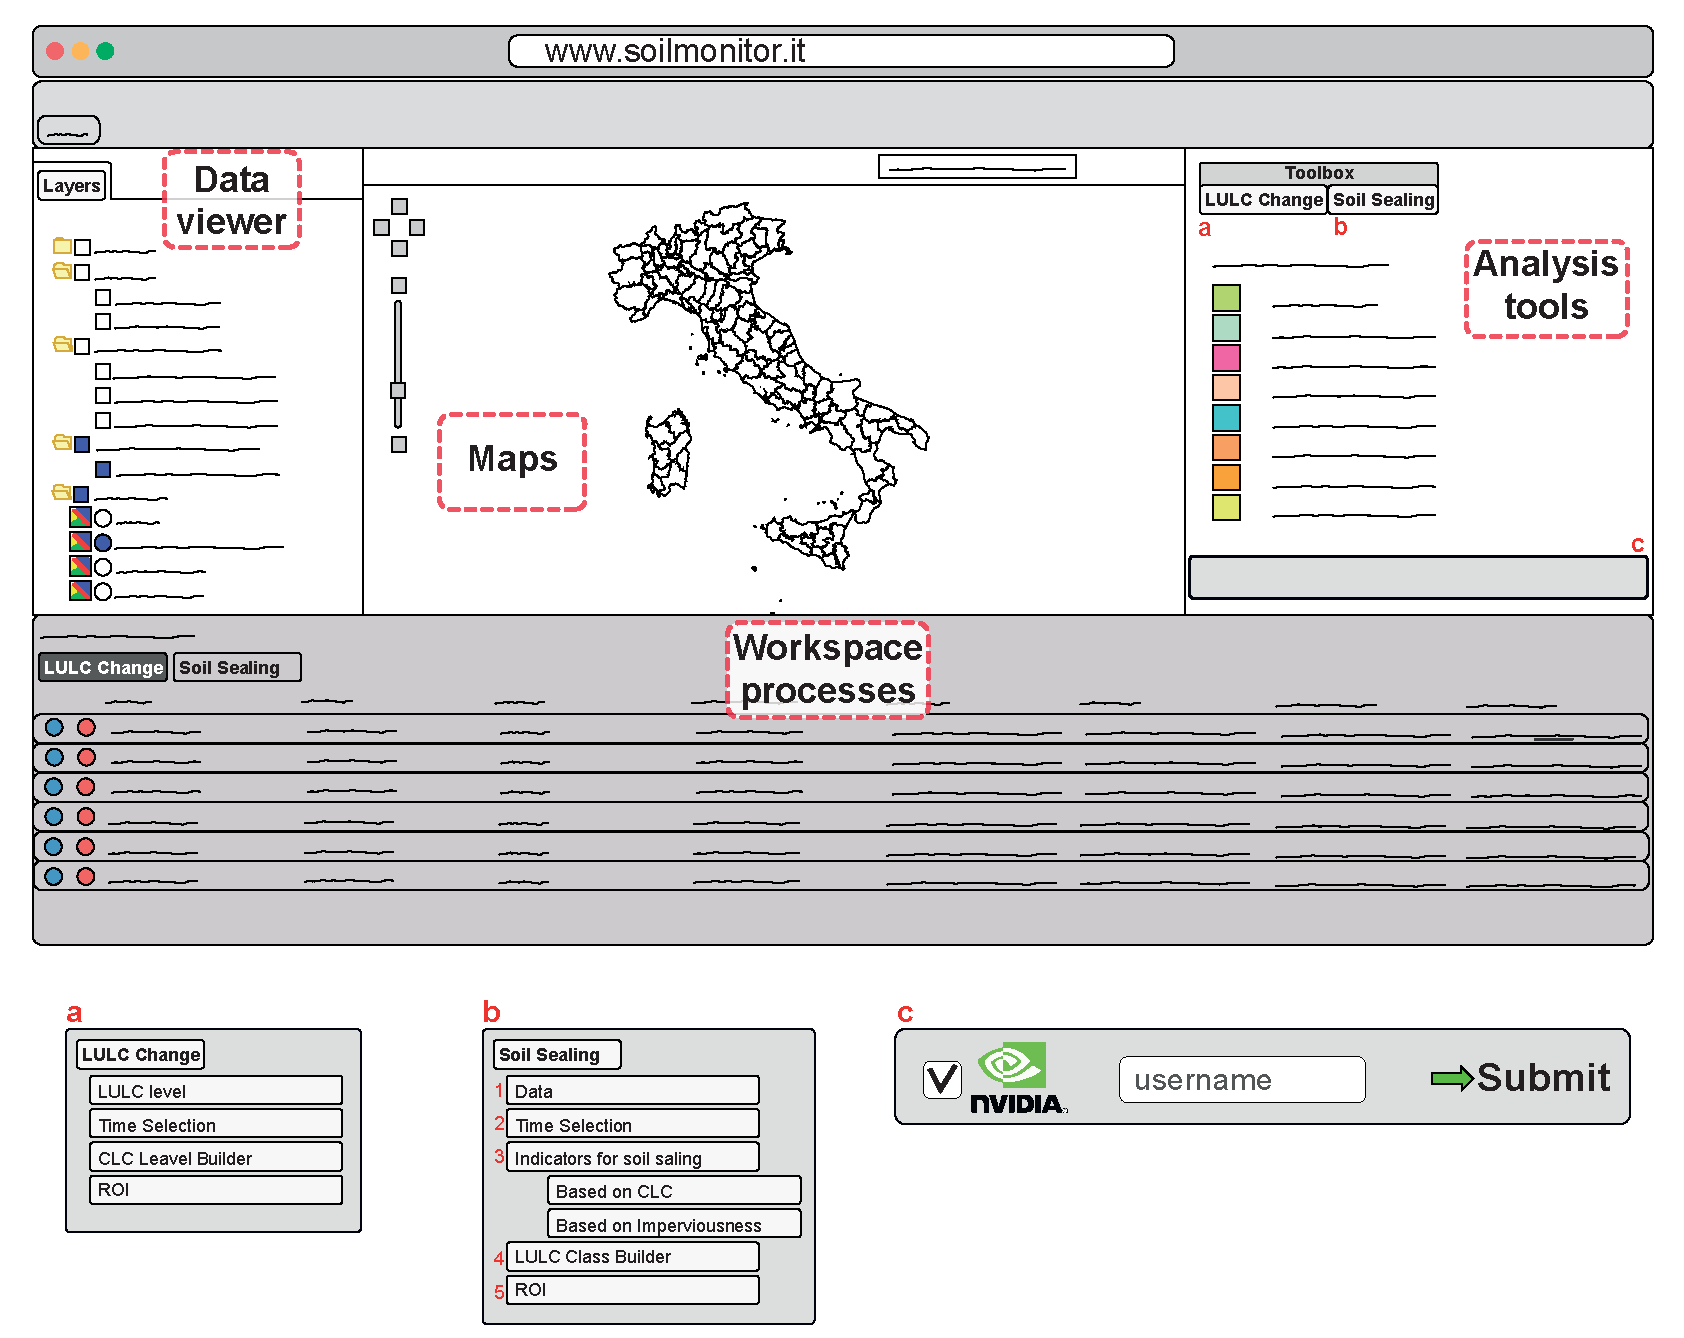
\includegraphics[width=500pt]{Figure01.pdf}}
    \caption{Exemplification of the Soil Monitor application (SMapp) dashboard with main panes (red boxes). 
    The user can build a tailored query owing to the job submission steps, one for the LULC change toolbox (a) and another one for the soil sealing toolbox (b). 
    Geospatial calculations can be distributed also on GPU cards owing to a tailored CUDA-C library developed for SMapp (c). } \label{fig:SMapp}
\end{figure}

SMapp is a three-tier logical architecture (Figure\ref{fig:GCI}) with separated processes made by (i) the \textit{visualization tier}, which displays information related to the services, (ii) the \textit{logic tier} that controls the functionality of the application by performing detailed processing, and (iii) the \textit{data tier}, which consists of the database where information is stored and retrieved in a manner that keeps data neutral and independent of the application servers and of the business logic.

\begin{figure}[t]
    % \includegraphics[width,,height=15pc,draft]
    % trim=left bottom right top, trim=0 0 0 50,clip,
    \centerline{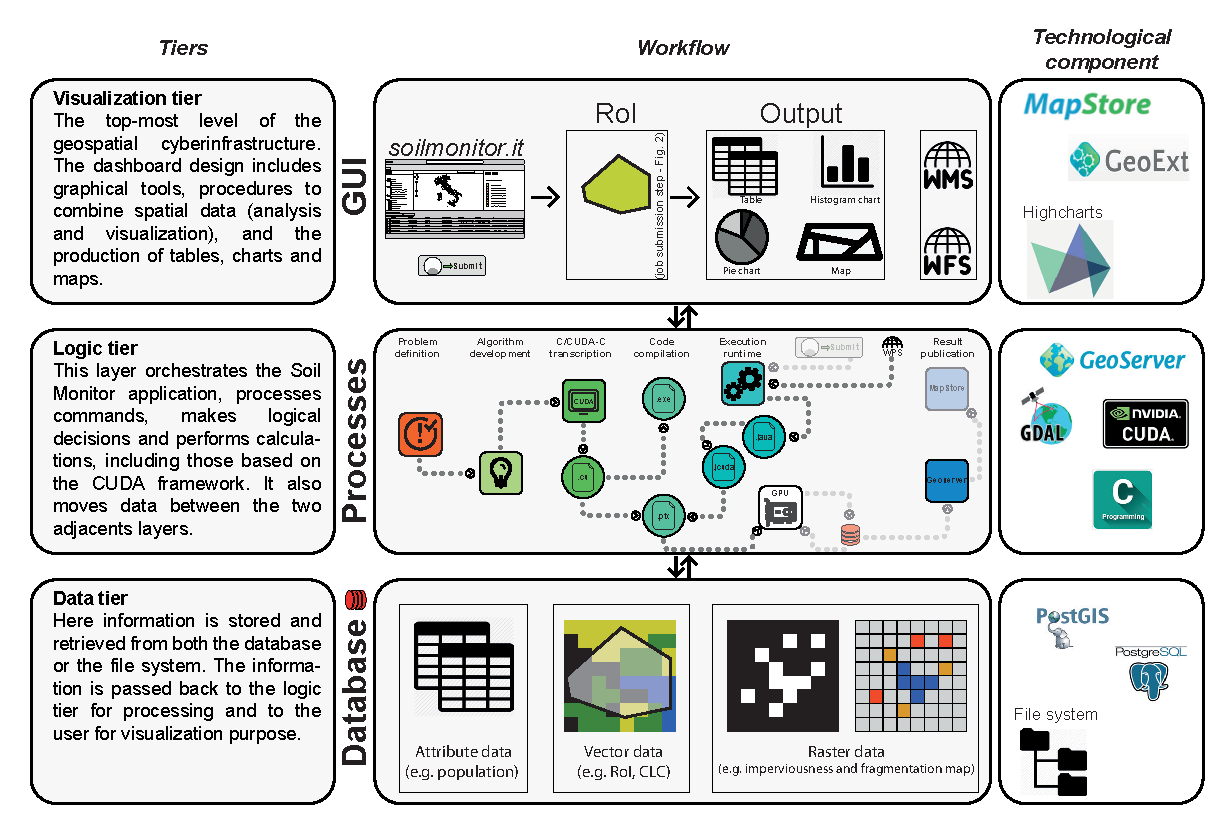
\includegraphics[width=500pt]{Figure02.pdf}}
    \caption{Main tiers, workflows, and technological components of the SMapp geospatial cyber infrastructure.} \label{fig:GCI}
\end{figure}

In Figure \ref{fig:GCI}, a synthesis is sketched of the operating mode of the platform showing the flow of data that feed different server functions (e.g. models), which, in turn, produce a set of services that can finally be accessed by the dashboard.

\subsection{Data layer}
The Open Geospatial Consortium (OGC), which aims to develop community-consensus open geospatial standards, provides a family of enabling technologies for sharing geospatial data and analytical capabilities on a distributed network. 
Data sharing (interoperability) in Soil Monitor is supported both in input --- to visualize data coming from remote services (such as ISPRA or other national level administrative bodies) --- and in output to provide different data services such as WMS and WFS to allow a client visualization of static images for instance over the desktop computer in GIS environments.
Moreover, web services are automatically appended to the new GIS data calculated by the CUDA engine to enable the visualization of results both locally within Soil Monitor, and remotely, for instance, within desktop GIS software environments.
Indeed, after ingestion in GeoServer, data become available for visualization and calculation purposes for the whole Italian territory Soil Monitor stores as follows:
\begin{itemize}
    \item The land use and land cover map in the period of 1956-60 produced by the Italian Touring Club in collaboration with National Council of Research, CNR (map of land use in Italy, scale 1: 200.000).
    \item The CORINE Land Cover (CLC) is a valuable source of information about land use and land cover, produced at the European level since the '90s and updated regularly (originally coordinated by the European Commission and the European Environmental Agency; now included in the Copernicus framework).
    CLC vector data are produced by photointerpretation of satellite images, with a minimum mapping unit of 25 ha and a classification system organized in three levels of thematic detail: level 1 with 5 land use and land cover classes, level 2 with 15 land use and land cover classes, and level 3 with 43 land use and land cover classes. 
    In SMapp, the raster version of CLC with a spatial resolution of 100 m is available for the years 1990, 2000, 2006, 2012, and 2018. Considering the homogeneity over the entire Europe and the constant update, CLC is largely used for spatial analysis, land cover change assessment, and policy making.
    \item The National High-Resolution Soil Consumption (NHRSC) was produced for Italy by ISPRA (ISPRA, 2016); the NHRSC is a raster that identifies artificial land cover areas with a spatial resolution of 10 m, produced for 2006, 2009, 2012, 2015, 2016, 2017 and 2018 with a semi-automatic classification of satellite images and the integration of local ancillary data such as OpenStreetMap; NHRSC included in Soil Monitor has a binary classification system such as non-sealed soil and sealed soil, according to the description given in Table \ref{tab:IMPclasses}.
    \item The administrative units: Italian administrative data are provided by the national institute of statistics (ISTAT). 
    These data represent the administrative units (also NUTS) in vector format.
    \item The population: population data are provided at the Municipal level by ISTAT, which periodically collects census data and updates this information every year. 
    \item The digital soil grids: Predictions on key soil properties performed globally at 250 m spatial resolution by ISRIC\footnote{available at http://data.isric.org/geoserver/sg250m/wms}. This is an example of interoperability based on the OGC standard called Web Mapping Service (WMS).
\end{itemize}

\begin{table}
\caption{Legend of the NHRSC map}\label{tab:IMPclasses}
\centering
\begin{tabular}[t]{ l l | l } 
\hline
\textbf{Code} & \textbf{Description} & \textbf{Classes} \\
\hline
\multirow{9}{4em}{0} & \multirow{9}{10em}{Non-sealed soil} & Tree/shrubs \\ 
 &  & Crops \\ 
 &  & Grassland \\ 
 &  & Water bodies \\ 
 &  & Wetlands \\ 
 &  & Rocks, beaches, and dunes \\ 
 &  & Glaciers and perpetual snow \\ 
 &  & Sport areas (pervious surface) \\ 
 &  & Other pervious surfaces \\ 
\hline
\multirow{10}{4em}{1} & \multirow{10}{10em}{Sealed soil} & Buildings \\ 
 &  & Road/Squares/Parking \\ 
 &  & Railway sites \\ 
 &  & Airports and ports (impervious surfaces) \\ 
 &  & Impermeable areas in sports fields \\ 
 &  & Permanent greenhouses \\ 
 &  & Solar farms on land \\ 
 &  & Mining areas \\ 
 &  & Dump sites \\ 
 &  & Other impervious areas \\
\hline
2 & Unclassified & \\
\hline
3 & Area outside the national boundary & \\
\hline
\end{tabular}
\end{table}

The CLC and Touring layers have been rasterized into 8-bit 100 meters resolution images to enable the grid-based calculations based on the CUDA framework.
Comparisons between CLC layers can be executed at three different levels of the legend detail (Level 1, Level 2, and Level 3) having different numbers of land use and land cover classes. 
In order to enable comparison with the Italian Touring Club layer, the most detailed CORINE legend (Level 3) has been homogenized with that from Touring Club. 
The imperviousness layers have been binarized (2-bit images) by applying a threshold to the level of imperviousness equal to 30\%, above which a pixel is taken as impervious.


\subsection{Visualization layer}
The dashboard design includes graphical tools, procedures to combine spatial data (analysis and visualization), and the production of tables and maps. 
The frontend application is based on MapStore (Figure \ref{fig:GCI}) and the overall structure of the graphical user interface can be distinguished in four main panes: the data, the map, the workspace, and the accordion panes (Figure \ref{fig:SMapp}).
The \textit{data pane} enables the visualization of different data, but not all information used in the calculation is visible, such as the population vector data. 
Moreover, MapStore enables users to add external data sources equipped with web services for rendering rasters and vectors, enhancing the overall interoperability of the platform. 
For instance, it can be particularly useful to compare the result of calculations with constraint maps coming from other data providers, such as the Italian Ministry of Cultural and Environmental Heritage, to check the soil sealing results. Furthermore, the \textit{map pane} enables the visualization of both the input geospatial data and the output maps calculated by the models and indicators available in the toolboxes. 
Moreover, the \textit{workspace pane} is where all instantiated requests are displayed. 
The toolboxes enable the allocation of several asynchronous requests per single user at the same time, which means that they can be calculated concurrently on the available CPU and GPU resources. 
The processes launched by users, which may be running at the same time, are displayed in the workspace as running, completed or interrupted according to their states. 
The \textit{accordion panes} are used to give the user full access to the processing layer parameters in a transparent way (see Figure \ref{fig:SMapp} for the query building procedure).

In addition to standard open-source codes available from the dual infrastructure GeoServer and MapStore, additional codes have been written to enrich functionality. 
For example, the client side has a dedicated interface to configure the RoI, which includes different methods such as the multiple selection of several administrative units at any hierarchical level (municipalities, provinces, and regions). 
Another example is given by the availability of different types of plots that are generated dynamically in addition to the geodata in order to enhance the readiness and interpretation of results.

\section{ \add[GL]{Results} }
\subsection{Processing layer}
On the server side, specific classes written in Java and CUDA have been developed to perform the calculations required to account for soil sealing and land take. 
Some calculations may be very demanding since they rely on high resolution grids (i.e. a square pixel of size 20 m) or on high thematic detail (i.e. CLC Level 3) feeding requests over large geographical areas (such as administrative regions or the whole Italy). For instance, this is the case of the rural fragmentation index, which is computed on the 20 m imperviousness layers. 
Even when selecting a small RoI, the relative high calculation demand depends on the logic of the algorithm itself, since it has to visit more than six thousand neighbour pixels $\left( \sim ( 800/\left(20\times2\right) )^2 \right)$ to calculate how fragmented each target pixel is, given a radius of 800 meters in the moving window selected by the user.
These cases may not manage to return answers in real-time or near-real-time for relatively large geographical extents, which explains one of the reasons why calculations are instantiated asynchronously.

In addition to data services, Soil Monitor implements Web Processing Services (WPS), which expose the algorithm of a soil sealing model or indicator outside the web application (Fig. 2). 
This was particularly useful to perform tests about the goodness of calculations in different spatial and temporal contexts, without the tedious infilling of the accordion panes to submit more and more requests. 
The test was performed by invoking a geospatial process with a known set of parameters by means of the supported POST request method submitted directly to the GeoServer endpoint. 
Subsequently, the parameters are passed to JCUDA, which, in turn, invokes the execution of CUDA kernels compiled in PTX files. 
The POST requests can be submitted from within the Unix terminal and, in our work, from MatLab scripts specifically designed for testing purposes. 
The testing procedure collects the results coming from the three independent computing environments: 
(i) the stand-alone executable (EXE) compiled from the source CUDA-C code; 
(ii) the WPS based on the JAI-JCUDA-CUDA chain executing the PTX compiled from the same source code used in the previous point; and 
(iii) a MatLab code implementing an alternative algorithm to perform the same geospatial processing. 
The test ends with a comparison of results coming from the three approaches to check for both speed performance and accuracy. 
This procedure was used as a standard during the development stage in order to test for inaccuracies in either the CUDA algorithms targeted to geospatial processing or in the deployment of the computing chains.
Further, WPS can be easily adapted to enable the dynamic binding of geospatial processes to aid client needs, such as running a standardized algorithm on personal data.

The CUDA framework and its binding from Java is implemented in the processing layer, where a list of developed CUDA kernels are loaded as a library in the infrastructure. 
First, a library of CUDA kernels is written in C, which can be used both standalone and as a compilation in PTX. 
Further, the Parallel Thread Execution (PTX) is a low-level parallel thread execution virtual machine and instruction set architecture, which provides a stable programming model and instruction set for general purpose parallel programming. 
Moreover, the PTX instructions are optimized for and translated to native target-architecture instructions. 
Second, the very fundamental CUDA kernels compiled as PTX files work as primitives that are combined in the JCUDA layer to build the crafted algorithms to address the soil sealing geospatial calculations. 
The advantage of this type of orchestration is that new models and indicators that may be added in the Soil Monitor toolboxes can be implemented using the same library of CUDA kernels, while little development and coding is required. 
Accordingly, an example of the pyramidal architecture based on the CUDA kernels is presented in Figure\ref{fig:ccl}, describing the calculation of the discontinuous urban fabric surface ($S_{DUF}$) using a connected component labelling algorithm specifically developed for SMapp. 
This algorithm is made of 8 CUDA kernels and one thousand lines of code performing the labelling of a 2-bit high resolution impervious layer in a 64-bit layer of ordered labels, one for each distinct urban patch.
Consequently, after identification and labelling, urban patches are sorted and then a threshold (90\%) is applied to extract only patches belonging to the discontinuous urban fabric. 
These patches are summed up to calculate the overall discontinuous urban fabric surface.

\begin{figure}[t]
    % \includegraphics[width,,height=15pc,draft]
    \centerline{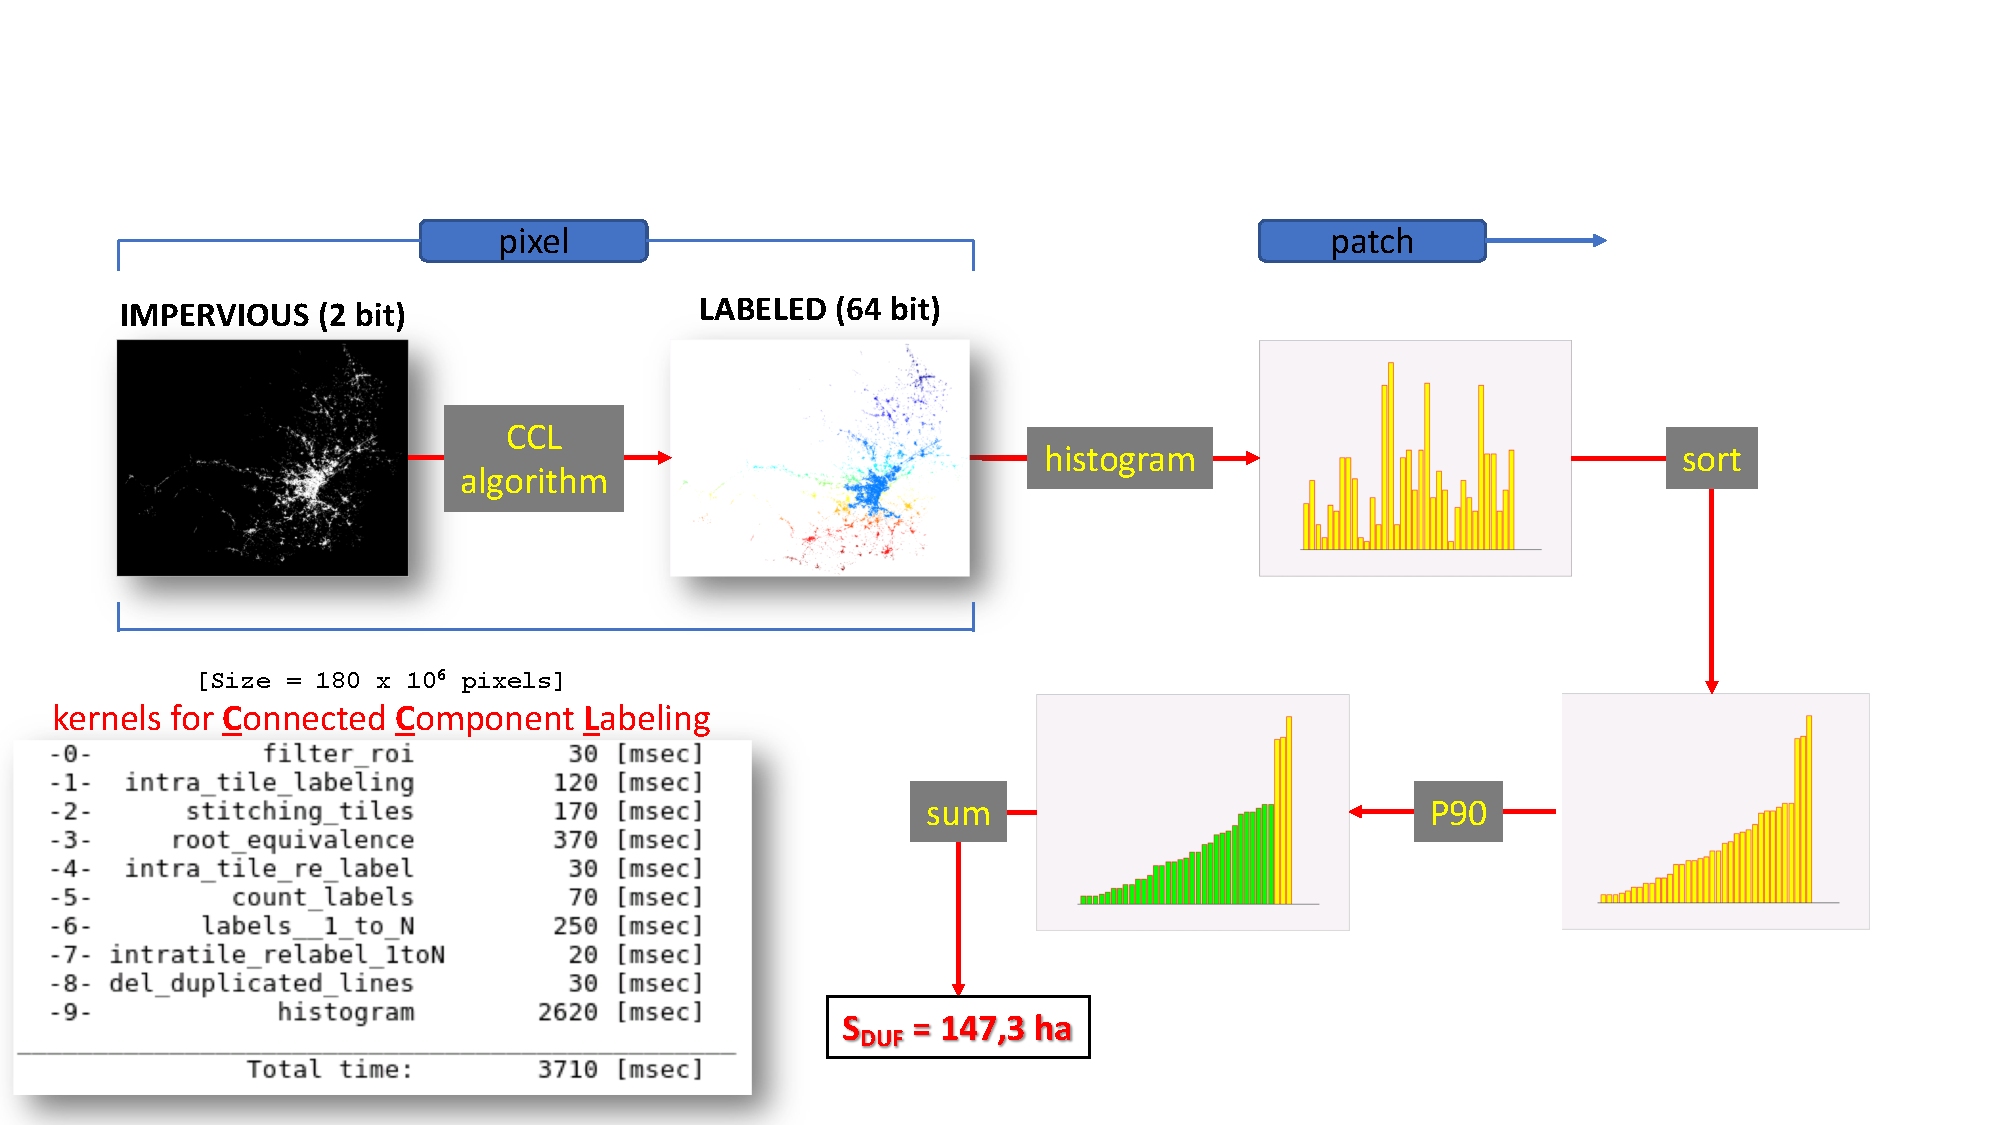
\includegraphics[width=500pt]{Figure03.pdf}}
    \caption{ The $S_{DUF}$ calculation developed in the CUDA framework within Soil Monitor GCI. 
    The pixel-based elaboration is solved by a connected component labelling algorithm written in CUDA-C. 
    Elapsed times in the kernel box refer to an image of size $180 \times 10^6$ pixels.} \label{fig:ccl}
\end{figure}


\subsection{Workflow of the integrated platform}
The integration of CUDA kernels, backend (i.e. Java and JCuda), and web interface requires a systematic workflow approach. 
A typical workflow includes three major steps: job submission, job status query, and results management, where the realization of each step requires integration across the three tiers of the cyberinfrastructure. 

Accordingly, Figure \ref{fig:SMapp} shows an overview of the available toolboxes for analysis, i.e. the toolbox for land use/land cover (LULC) change (Figure \ref{fig:SMapp}, a) and the toolbox for soil sealing indicators (Figure \ref{fig:SMapp}, b).
The user can build a tailored query owing to the two job submission steps, one for each toolbox. 
For any soil sealing indicator, the user must select --- according to the following hierarchical order --- the dataset they intend to use (i.e. CORINE land cover or high-resolution imperviousness layer, Figure \ref{fig:SMapp}, b1); the time of the analysis (one year or two years, Figure \ref{fig:SMapp}, b2); the selection of a soil sealing indicator (Figure \ref{fig:SMapp}, b3); the composition of LULC classes optionally (Figure \ref{fig:SMapp}, b4); and finally, the region of interest (Figure \ref{fig:SMapp}, b5). Therefore, in order to ease the definition of a possible multi-polygon RoI, there is an ad hoc accordion pane for the rapid identification and selection of any Italian administrative unit.
The RoI definition accordion pane is particularly useful because it allows the user to select one or more administrative units at any level of the topological hierarchy (municipality, province, region) and to freely draw a new region of interest directly over the displayed map within SMapp.
For any subsequent query to the first one, the user can change only the parameters strictly required for the new job submission (e.g. change the indicator or the time) and SMapp will calculate the new indicator given the parameter set just defined. 
This behaviour was expressly required by end users to facilitate the instantiation of more requests for the purpose of scrutinizing the implementation of executed urban plans.

\subsection{Description of models/indicators of soil sealing}
The list of indicators we have developed and implemented are given in Table 2, which have been chosen in close collaboration with urban planners to address their planning needs. 
They refer to land use/land cover descriptors, rate of change of land use/land cover, marginal soil sealing, extent of urban sprawl, density of urban boundaries, degree of urban dispersion, rural/urban fragmentation, global land take dynamics, and estimate of loss in food supply due to soil sealing. 
The table refers to the two official datasets described above, i.e. the Corine Land Cover and the soil imperviousness. 
The CLC layers allow investigations on multiple classes of land use and land cover but at a relatively coarser spatial resolution (either 100 m or 250 m spatial resolution).
Conversely, soil imperviousness is available over high spatial detailed layers (20 m spatial resolution) and aggregates the information of land use in only two classes, i.e. sealed and unsealed land. 
Furthermore, the choice between the two datasets reflects the kind of soil sealing indicator, the detail in the thematic domain, and the spatial resolution required in the output map. 


\begin{table}[b]
    \caption{ Models in SMapp toolbox for soil sealing and land take. }
    \label{tab:SMappToolbox}
    \small
    \centering
    \begin{tabular}{m{0.3cm} p{0.1cm} p{1.2cm} p{3.5cm} *{3}{p{2.7cm}} p{1.0cm} }
    
    \toprule
        & \textbf{ID} & \textbf{Model} & \textbf{Formula$^\dagger$} & \textbf{Description} & \textbf{Application} & \textbf{Techonological Novelty} & \textbf{Outputs}\\
    \midrule\midrule
    
    \multirow{5}{*}{ \rotatebox[origin=c]{90}{ \shortstack[c]{ Calculation using LULC rasters at 100m spatial resolution \\ (e.g. CLC produced by Copernicus)} } } 
    & 0 & LULC & --- & Change of state of each LULC class from a reference year to a current year & Evolutionary traiectories & CUDA kernels producing both an interactive change matrix and a map of all changes & pie chart, vector map  \\
    
    & 1	& Coverage Coefficient & $\frac{S_{CLC_i}}{S_{AU}}$ & Fraction of total surface covered by i-th land use/cover class & Classes consistency within a user defined RoI (admin unit or free area) & None & bar chart, vector map \\
        
    & 2 & Rate of Change & 
    $\frac{ \left(S_{CLC_i}\right)_{T_2} - \left(S_{CLC_i}\right)_{T_1} }{ \left(S_{CLC_i}\right)_{T_1} }$ 
    & Rate of change of any i-th land use/cover class & Change of classes consistency within a user defined RoI (admin unit or free area) & None & bar chart, vector map \\
    
    & 3 & Marginal Land Take & 
    $\frac{ \left(S_{CLC_1}\right)_{T_2} - \left(S_{CLC_1}\right)_{T_1} }{ \left(POP_{au}\right)_{T_2} - \left(POP_{au}\right)_{T_1} }$
    & Ratio between urbanization variation and population growth variation between two years & Analyse variation of urbanization with respect to variation of population to depict temporal trends & None & bar chart, vector map \\
    
    & 4	& Urban Sprawl & 
    $\frac{ \frac{ \left(S_{CLC_1}\right)_{T_2} - \left(S_{CLC_1}\right)_{T_1} }{ \left(S_{CLC_1}\right)_{T_1} }  }     { \frac{ \left(POP_{au}\right)_{T_2} - \left(POP_{au}\right)_{T_1} }{ \left(POP_{au}\right)_{T_1} } }$
    & Ratio between urbanization rate and population growth rate between two years & Standardized version of marginal land take & None & bar chart, vector map \\
    
    \midrule
    
    \multirow{9}{*}{ \rotatebox[origin=c]{90}{ \shortstack[c]{Calculation using high resolution imperviousness rasters at 20m spatial resolution \\ (NHRSC produced by ISPRA)} } } 
    & 5 & Urban sprawl & 
    $\frac{S_{DUF}}{S_{UT}}$ 
    & Ratio between discontinuous urban fabric and total urban surface & To know the composition of urban development related to sprawl phenomenon, which can be related to fragmentation & Tailored connected component labeling algorithm in CUDA & bar chart \\
    
    & 6 & Edge Density (ED) &
    $\frac{P_{UT}}{S_{UT}}$ 
    & Ratio between perimeter and surface of urbanized ares in selected RoI & Density of urban margins, which is related to urban fragmentation & CUDA kernels computing both the perimeter and the urbanized area & bar chart \\
    
    & 7 & Urban Area &
    $\frac{S_{UT}}{S_{AU}}$ 
    & Fraction of total surface covered by urbanization & To know the magnitude of land take related to the administrative unit & CUDA kernels computing the urbanized area	& barchart \\
    
    & 8	& Largest Class Patch Index (LCPI) & 
    $\frac{S_{max}}{S_{UT}}$ 
    & Fraction of urban surface within the largest urban patch & Represents the level of compactness of the urban area & CUDA kernels computing the connected component labeling	& bar chart \\
    
    & 9	& Residual Mean Patch Surface (RMPS) &
    $\frac{S_{DUF}}{N_{DUF}}$ 
    & Average surface of all urban patches excluding the largest patch & Mean patch area within the discontinuous urban fabric, which can be related to urban texture & CUDA kernels computing the connected component labeling & bar chart \\
    
    & 10 & Rural/Urban Fragmentation &
    $\frac{\sum^{N}_{k=1} V_k}{ n-1 }$ 
    & Fraction of pixels having the same value of the center pixel in a mask & e.g. on rural center pixels it highlights ecological corridors & 1k lines of code; 6 CUDA kernels; 8 geospatial parameters & raster map \\
    
    & 11 & Land Take (and Gains) &
    $ \left( V_{pix} \right)_{T_2} - \left( V_{pix} \right)_{T_1}$ 
    & Difference of the value of a pixel between two differenr times & A map with three possible pixel values: (0) if no change occured; (-1) if land take; (+1) if land gain & Based on the basic reduce CUDA kernel & raster map, bar chart \\
    
    & 12 & Net Loss of Food Supply &
    $ \sum_{pix=0}^{image} \left( \left( V_{pix} \right)_{T_2} - \left( V_{pix} \right)_{T_1} \right) \times C $ 
    & --- & Potential loss of aggregated ecosystem function (coeff :: FAO) & Based on the basic reduce CUDA kernel & bar chart \\
    
    & 13 & Model of Urban Development & Composite of IDs 6, 8 and 9 & --- & ---	& Same as aggregating IDs 6, 8 and 9 plus a 3-D view highlighting urban development in both different administrative units and times & 3-D scatplot \\
    
    \midrule\bottomrule
    
    \multicolumn{8}{p{17.2cm}} % 13.9cm is the sum of all column previously defined by p{}
    {
      \footnotesize{$^\dagger$Definitions. 
      $S$:area;
      $P$:perimeter;
      $V$:value;
      $S_{CLC_i}$:area of $i_{th}$ CORINE Land Cover class at selected legend level; 
      $S_{AU}$: area of administrative unit; 
      $S_{CLC_1}$: area of urban CLC class at selected legend level; 
      AU: administrative unit (city, province, region, \ldots); 
      $T_1$: time before; 
      $T_2$: time after; 
      $POP_{AU}$: population within AU; 
      $S_{DUF}$: area of discontinuous urban fabric; 
      $N_{DUF}$: number of urban patches within discontinuous urban fabric; 
      $S_{UT}$: total urban area; 
      $V_k$: value of the pixel \textit{k} within the kernel of N pixels };
      $V_{pix}$:value of pixel in NHRSC raster;
      C: FAO coefficient equal to 0.6 $persons \times ha^{-1} \times year^{-1}$
      .
    }
    \end{tabular}
\end{table}

\subsection{Application: case studies with validation}
\subsubsection{The case study of Italy}
In Italy, the monitoring of land take is ensured by the National System for the Protection of the Environment (SNPA) as established by L.132/2016.
Accordingly, the SNPA is coordinated by ISPRA and involves all Italian Environmental Protection Agencies (ARPA-APPA). 
This monitoring is scheduled in order to have an annually updated picture of the soil sealing evolution (e.g. ISPRA 2016, 2018) and the dynamics of land transformation and urban development, which is done through the production of thematic maps and the development of specific indicators. 
The L.132/2016 states that the SNPA must ensure such monitoring through monitoring points/networks or earth observation techniques (e.g. Copernicus).
In performing such monitoring, ISPRA and SNPA face two major problems: (i) difficult interaction with over 8000 Italian municipalities and (ii) the lack of awareness about the crucial importance of the soil sealing land degradation process by citizens and other public authorities.

In this framework, Soil Monitor can indeed represent an important step forward in land take and land use monitoring.
Moreover, any administrative unit can monitor land take and land use/cover evolution through maps (e.g. showing the new urbanized area), numeric or graphical representation of some indicators, and comparing indicators between different years, for instance, to evaluate changes in urban development or in the fragmentation of the rural territory.

Furthermore, it is important to highlight that Soil Monitor contributes to the analysis of soil sealing through standardized approaches, thus avoiding the current trend of creating several customised indexes produced by many users as it currently happens in using the large flexibility offered by many kinds of desktop software (e.g. fragstat\footnote{https://www.umass.edu/landeco/research/fragstats/fragstats.html}). 

A case of use of the platform is given in Figure \ref{fig:caseIT}, where the matrix of land use and land cover changes (LULC) for all of Italy has been analysed and reported. 

\begin{figure}[t]
    % \includegraphics[width,,height=15pc,draft]
    \centerline{\includegraphics[width=450pt]{Figure04.pdf}}
    \caption{ The interactive change matrix for Italy between 1954 and 2012.
    The changes in both the chart and the map are depicted by colours, each of which is associated with the class in the reference year (1954) consumed by artificial surfaces in the current year (2012) } \label{fig:caseIT}
\end{figure}

Additionally, any RoI can be freely selected by the user and any portion (administrative levels included) of the Italian territory can be analysed. Consequently, the change matrix calculation is highly demanding due to the high number of classes that can be included (in particular, using CLC at Level 3), to the large spatial extent and the high spatial detail; therefore, a multi-GPU approach was developed, through CUDA streams, to further accelerate demanding requests thus enabling real-time queries. 
The system produces a table with all land use changes for two contrasting years. 
For instance, in Fig 4a, all the changes of state contributing to the \textit{artificial surfaces} class between two different years was selected. 
In our case, the largest land use class affected by new artificial surfaces is the \textit{complex cultivation patterns} class, with a loss of about 418 thousand hectares from 1954 to 2012. 
Accordingly, the key innovation in Soil Monitor consists of an interactive matrix of changes, which can be dynamically queried fixing a column (i.e. class of \textit{artificial surfaces} in 2012) or a row (i.e. a class of any other land use in 1954), getting a chart and a map of changes on demand. 
Moreover, a pie diagram provides an immediate quantification of the changes by classes contributing to \textit{artificial surfaces} (Figure \ref{fig:caseIT}b). 
The map depicts the geography of changes providing details till the pixel level; it is possible to observe that the largest changes from complex cultivation patterns to artificial areas occurring at the fringes of earlier urban centres (Figure \ref{fig:caseIT}c). 
This geospatial analysis, especially when used to compare and analyse LULC changes between more recent years, is a very powerful tool. 
It provides very detailed geospatial information about the land use classes, which have been affected more by urbanization, and it possibly highlights those LULC classes that have a major risk to be affected by new urbanization in the near future. 
Further, the new urbanization depicted in Fig. 4c shows that the land use mostly affected by urbanization is the less specialised one, namely \textit{complex cultivation patterns}. 
Therefore, higher specialization in agriculture would perhaps produce more resilient LULC classes to challenge new land take pressures.

\subsubsection{The case study of territorial plan (PTCP)}
In Italy, the reference administrative level for urban planning coordination in terms of environmental issues is the province law 142/1990. 
Thus, it is the key geographical level to challenge land take. 
However, this situation somehow remained unchanged after law 56/2014 (rules on metropolitan cities) and even after the constitutional referendum that transfers the competences of the provinces to the regions (4 December 2016).
Currently, provinces (albeit in specific cases, metropolitan cities and regions) carry out the fundamental coordinating role for territorial planning, protection, and enhancement. 
Moreover, typically, this is performed through the ''territorial plan of coordination at province level'' called PTCP (Piano Territoriale di Coordinamento Provinciale), which aims at: (i) land use regulation to protect natural areas and cultural heritage; (ii) guidance and implementation of subordinate planning producing general guidelines to be followed by municipalities in their local plans; (iii) coordination of planning activities by local authorities in order to achieve a rational organization of the provincial spaces.

In the last decades, there have been many regional laws and provincial policies in Italy, highlighting the need to mitigate land take, thus guaranteeing the preservation of the landscape and its ecosystem services. 
In such a framework, the crucial need to support the PTCP planning in order to truly mitigate soil sealing is evident. 
This government level is farther to the pressures  of pro-growth policies, which are instead strongly grounded in the city and town leading coalitions.
Therefore, Soil Monitor can help implement these regulative ambitions.
For each Italian province, the platform allows carrying out a detailed analysis of both recent and past urbanization with the production of indices and maps identifying the main soil sealing criticalities within the territory.
Moreover, Soil Monitor classifies administrative units on the base of urban sprawl, giving the opportunity to the governing body to define targeted and selected geographies of the densification policy.

A case of use of the platform at the provincial level is reported in Figure \ref{fig:casePROV}, which shows a plot of three indicators, namely LCDI, RMPS, and ED (presented in Table \ref{tab:IMPclasses}), describing the model of urban development of the five provincial capitals in Campania Region: Avellino, Benevento, Caserta, Napoli, and Salerno (Figure \ref{fig:casePROV}a). 
The combination of the results of the three indicators helps in evaluating the degree of urban dispersion and, for instance, enables differentiating monocentric from polycentric municipalities. 
As such, Caserta, Napoli, and Salerno --- having a LCPI larger than 70\% --- are monocentric and compacted, while Avellino and Benevento have a clearly polycentric distribution.

\begin{figure}[t]
    % \includegraphics[width,,height=15pc,draft]
    \centerline{\includegraphics[width=250pt]{Figure05.pdf}}
    \caption{ Soil Monitor supports the analysis at the level of the territorial plan of coordination (PTCP). } \label{fig:casePROV}
\end{figure}

In Figure \ref{fig:casePROV}b a quantitative map of the rural fragmentation is given for the Milano province, an area very dynamic with a high per capita income and high residential and infrastructure pressure. 
This map is very important because it enables the quantification of each point in the landscape to the degree of its rural integrity. 
Accordingly, calculations are performed on-the-fly, enabling the planners to freely decide the radius of their analysis (size of kernel to be processed).
Generally, a smaller radius (e.g. 100 m) is useful for detailed urban planning at the scale of a specific intervention, such as a new green corridor or a new development.
By contrast, a fragmentation analysis performed with a large radius (e.g. >500 m) produces an output affected by very large areas, either urban or natural. 
Thus, this analysis is useful to describe major geographical trends of rural integrity.

The output from the above analysis can be profitably used to better plan future urban development, thus avoiding new fragmentation of rural areas, especially those with high integrity, and to plan where to place new green infrastructures connecting rural areas with high rural integrity.

\subsubsection{The case study of the municipal plan (PUC)}
The municipal urbanization plan (PUC) is a tool for the management of the Italian municipal territory, which consists of cartographic and technical documents along with regulations for the management of urban and territorial transformations within the municipality.

The PUC stems from the old well known general regulatory plan (PRG established by Italian law 1150/1942); it is produced by urban planners assisted by experts from other fields (e.g. environmental scientists, pedologists, geologists, and lawyers).

Therefore, the PUC must have a long series of requirements: (i) the identification and discipline of land uses; (ii) the subdivision of the territory into zones with different and complementary uses; (iii) the protection and enhancement of natural, landscape, and historical-cultural heritage. 
Although the PUC has no duration limitations, it is periodically reviewed.
Moreover, since the PUC is the planning document closer to operational urban activities, it is important for Soil Monitor to be used at this scale. 
At the municipal scale, Soil Monitor enables performing a scenario analysis by simulating different urban interventions of green corridors by evaluating the effects of such interventions on the rural integrity; the system also allows the visualization and connect planning information with other environmental maps such as landscape constraints.

\begin{figure}[t]
    % \includegraphics[width,,height=15pc,draft]
    \centerline{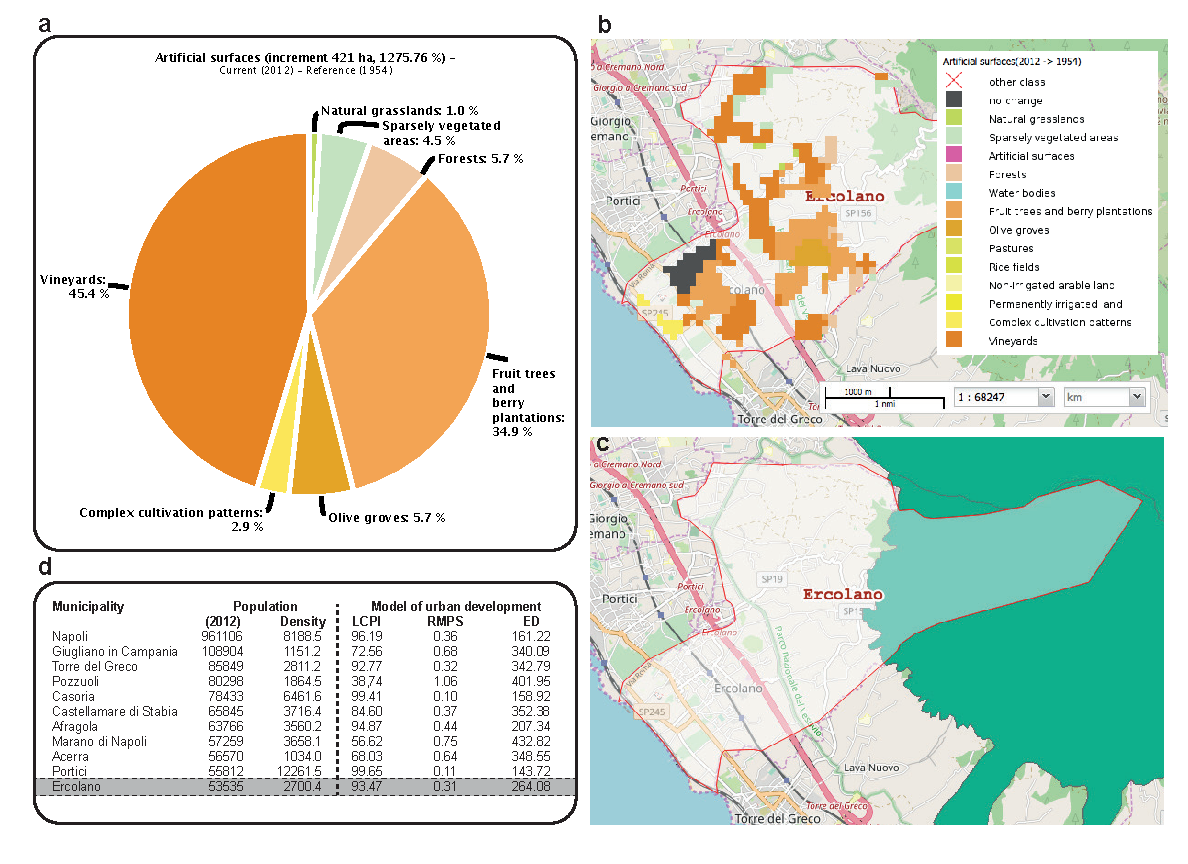
\includegraphics[width=450pt]{Figure06.pdf}}
    \caption{ Soil Monitor supports the analysis at the level of the municipal urbanization plan (PUC). } \label{fig:caseCOM}
\end{figure}

A case of use of the platform at the municipality level is reported in Figure \ref{fig:caseCOM}. 
The city of Ercolano is located between the Vesuvius volcano and the sea, has a high population density, and is devoted to tourism owing to historical sites and spot of high-quality agriculture (e.g. wine, fruit trees, and flowers). 
Therefore, the user can get a quantification of the evolutive trajectories that led to specific land use and land cover states. 
In the example shown in Figure \ref{fig:caseCOM}(a, b), the amount and the geolocation of the consumption exerted by artificial surfaces is clear, above all, regarding vineyards, fruit trees, and olive orchards. 
This interpretation about the LULC evolution is accompanied by the recognition that part of the land take was very close (if not inside) to the protected areas (Figure \ref{fig:caseCOM}c) of the Vesuvius's slopes, thereby confirming the very high pressure of urbanization not well managed by local authorities.
Accordingly, the model of urban development was computed in the same municipality of Ercolano against other most populated cities in the Napoli province. 
Figure \ref{fig:caseCOM}d shows the population size and density (the left side of the table) and the indicators of model of urban development (LCPI, RMPS, and ED on the right side of the table), depicting the main urban trends in the Napoli province. 
The results reported in Figure \ref{fig:caseCOM} are limited examples of the information that can possibly be achieved using Soil Monitor, which can be profitably used to enhance the definition and implementation of plans at the municipality scale (PUC in Italy). 
This finding becomes much more important considering Soil Monitor is operational over the entire Italian territory with more than eight thousand municipalities.

\section{Conclusions}
Soil sealing mitigation implemented through best land spatial planning practices is a very virtuous goal, but it is also one of the greatest challenges of the modern world. 
In fact, high quantity of information can only be accessed through satellite and drones, etc. concerning, for example, the agricultural, forestry, environmental, and spatial planning sectors is simply not sufficient to face the complexity of this challenge.

This work shows that starting from the problem statement in a specific research domain, it is feasible to combine recent achievements in terms of data, models, indicators, WebGIS, and HPC technologies to produce an integrated geospatial cyberinfrastructure available on the web, aiming to account and mitigate the continual soil sealing worldwide. 
The proposed application called SMapp, which is freely accessible via an internet browser without the need to install any application or plugin on the local computer, aims to demonstrate that this approach is feasible. 
Moreover, it takes advantage of the combination of updated high spatial resolution data on imperviousness available in Italy owing to ISPRA with tailored codes written in CUDA to gain embarrassingly parallel applications, thereby enabling a highly detailed analysis over large geographical extents.
Additionally, the combination of WebGIS with GPU computing running on-the-fly geospatial processing puts Soil Monitor at the fringe of research and development. 
Further, the GPU parallelism model enables a higher speedup than the CPU counterpart, at both a lower cost and a lower power consumption, with the main limitation being the requirement to design and write new codes from scratch.

Nevertheless, the proposed platform still remains a prototype from research that can be used for any area of the Italian territory. 
Subsequently, it can be seen as a democratic tool for creating reports that can catch the evolution of land use trajectories and connected land degradation interpretations about the ongoing land degradation processes.

Despite the above positive statements, it is also essential to underline that the construction, maintenance, and updating of the infrastructure requires the following:
\begin{enumerate}[label=(\roman*)]
    \item Above all, a more comprehensive and detailed data on soils which, at least in Italy, are still missing to account for land degradation surface quantity. 
    This information is critical to discriminate between the different land qualities vulnerable to land take. 
    As such, we put soil grids by ISRIC via WMS to smoothly mitigate this fundamental shortcoming, considering the low accuracy of this grid with respect to the scale and detail of the land take accountancy.
    \item A strong scientific effort to find the most suitable and reliable approaches for each application considering the available data.
    \item A strong effort to integrate different types of knowledge and technology to develop and implement web applications, according to the use of open-source components such as GeoServer and MapStore.
    \item Strong technical work to make the tools fully operational, mainly because of the need to provide real time answers (e.g. \textit{what-if} modelling and scenario analysis).
    \item The need for the constant maintenance of data and applications in order to keep the platform constantly and consistently operational and not obsolete.
    \item To reinforce the interoperability with data shared by other official providers. 
    The more data and thematic layers available, the higher strength of deductions and interpretations performed during the analysis.
    \item A more intuitive dashboard to simplify the user interaction with the visualization layer.
    Indeed, because of the money constraints during the development, Soil Monitor does not ensure an easy and intuitive navigation during the job submission step. 
    Nevertheless, we recognized the importance of a future effort to enhance fruition.
\end{enumerate}

Soil Monitor, by placing emphasis on landscapes, seeks to reduce the gap between policy and implementation being able to quantify and visualize (with the change in time of) the state of the land system.

\section*{ORCID}
Giuliano Langella \href{https://orcid.org/0000-0001-7210-0906}{ {\orcidicon{0000-0001-7210-0906}}\hspace{1.0mm} orcid.org/0000-0001-7210-0906}


\bibliography{SMapp}

%The normal commands for producing the reference list are:
%\begin{verbatim}
%\begin{thebibliography}{99}
%\bibitem{<x-ref label>}
%         <Reference details>
%\end{thebibliography}
%\end{verbatim}

\end{document}